The counterexamples for general surveillance properties are directed graphs, which may contain cycles. In particular, for a liveness surveillance property of the form $\LTLglobally\LTLfinally p_k$ each infinite path in the graph has a position such that, from this position on, each state on the path violates $p_k$. An \emph{abstract counterexample graph} in the game $(G_\abstr,\LTLglobally\LTLfinally p_k)$ is a finite graph $\counterex_\abstr$ defined analogously to the abstract counterexample tree. The difference being that there are no leaves, and that for each cycle $\rho = v_1,v_2,\ldots,v_n$ with $v_1 = v_n$ in $\counterex_\abstr$ that is reachable from $v_0$, every node $v_i$ in $\rho$ is labelled with state $s_\abstr^i$ where $s_\abstr^i \not\models p_k$.
%\begin{itemize}
%\item There exists a node $v_0$ of $\counterex_\abstr$ labelled with $s^\init_\abstr$.
%\item For each cycle $\rho = v_1,v_2,\ldots,v_n$ with $v_1 = v_n$ in $\counterex_\abstr$ that is reachable from $v_0$, every node $v_i$ in $\rho$ is labelled with state $s_\abstr^i$ where $s_\abstr^i \not\models p_k$.
%\item The graph branches according to all possible transition choices of the agent. Formally, if a node $v$ is labelled with $(l_a,A_t)$, then there exists an $A_t'$  such that: (1) $((l_a,A_t),(l_a',A_t')) \in \trans_\abstr$ for some $l_a' \in L_a$, and (2) for every $l_a' \in L_a$ such that $((l_a,A_t),(l_a,A_t')) \in \trans_\abstr$, there is a child $v'$ of $v$ labelled with $(l_a',A_t')$.
%\end{itemize}   

\begin{figure}
\begin{minipage}{0.2\textwidth}
\begin{center}
%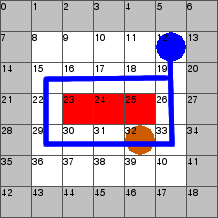
\includegraphics[scale=.33]{figs/7x7_liveness.png}
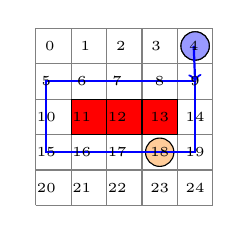
\begin{tikzpicture}[scale=0.9]
\draw[step=0.5cm,color=gray] (-1.5,-1.5) grid (1,1);
\filldraw[fill=blue,draw=black] (+0.75,+0.75) circle (0.2cm);
\filldraw[fill=red,draw=black] (0,0) rectangle (-0.5,-0.5);
\filldraw[fill=red,draw=black] (-0.5,0) rectangle (-1,-0.5);
\filldraw[fill=red,draw=black] (0,0) rectangle (0.5,-0.5);
\filldraw[fill=blue!40!white,draw=black] (+0.75,+0.75) circle (0.2cm);
\filldraw[fill=orange!40!white,draw=black] (0.25,-0.75) circle (0.2cm);
\draw[blue,thick] (-1.35,-0.75) rectangle (0.75,0.25);
\draw[blue,thick,->] (0.73,0.75) -> (0.75,0.25);
\node at (-1.30,+0.75) {\tiny{0}};
\node at (-0.80,+0.75) {\tiny{1}};
\node at (-0.30,+0.75) {\tiny{2}};
\node at (0.20,+0.75) {\tiny{3}};
\node at (0.73,+0.75) {\tiny{4}};
\node at (-1.35,+0.25) {\tiny{5}};
\node at (-0.85,+0.25) {\tiny{6}};
\node at (-0.35,+0.25) {\tiny{7}};
\node at (0.25,+0.25) {\tiny{8}};
\node at (0.75,+0.25) {\tiny{9}};
\node at (-1.35,-0.25) {\tiny{10}};
\node at (-0.85,-0.25) {\tiny{11}};
\node at (-0.35,-0.25) {\tiny{12}};
\node at (0.25,-0.25) {\tiny{13}};
\node at (0.75,-0.25) {\tiny{14}};
\node at (-1.35,-0.75) {\tiny{15}};
\node at (-0.85,-0.75) {\tiny{16}};
\node at (-0.35,-0.75) {\tiny{17}};
\node at (0.25,-0.75) {\tiny{18}};
\node at (0.75,-0.75) {\tiny{19}};
\node at (-1.35,-1.25) {\tiny{20}};
\node at (-0.85,-1.25) {\tiny{21}};
\node at (-0.35,-1.25) {\tiny{22}};
\node at (0.25,-1.25) {\tiny{23}};
\node at (0.75,-1.25) {\tiny{24}};
\end{tikzpicture}
\end{center}
\end{minipage}
\begin{minipage}{0.28\textwidth}
\vspace{0.1cm}
\caption{\small Agent locations on an (infinite) path in the abstract counterexample graph from Example~\ref{ex:simple-liveness-counterex}. In the graph, the first node is labelled with $(4,18)$, the second with $(9,\{Q_2\})$, and all other nodes with some $(l_a,\{Q_1,Q_2\})$.}
\label{fig:simple-liveness-counterex}
\end{minipage}
\vspace{-.65cm}
\end{figure}

\begin{example}\label{ex:simple-liveness-counterex}
We saw in Example~\ref{ex:simple-safety-realizability} that in the safety surveillance game $(G,\LTLglobally p_2)$ the agent does not have a winning strategy. %This means, that the agent cannot ensure keeping at all times the uncertainty about the current position of the target to at most two positions.
We now consider a relaxed requirement, namely, that the uncertainty drops to at most $2$ infinitely often. We consider the liveness surveillance game 
$(G,\LTLglobally \LTLfinally p_2)$.

Let $\part = \{Q_1,Q_2\}$ be the partition from Example~\ref{ex:simple-safety-unconcretizable}. %that is, $Q_1$, corresponds to the first two columns of the grid in Figure~\ref{simple-grid} and the set $Q_2$ contains the locations from the other three columns of the grid. 
Figure~\ref{fig:simple-liveness-counterex} shows an infinite path (in lasso form) in the abstract game $(\alpha_\part(G),\LTLglobally \LTLfinally p_2)$.  The figure depicts only the corresponding trajectory (sequence of positions) of the agent. The initial abstract state is $(4,18)$, the second node on the path is labeled with the abstract state $(9,\{Q_2\})$, and all other nodes on the path are labeled with abstract states of the form $(l_a,\{Q_1,Q_2\})$. As each abstract state in the cycle violates $p_2$, the path violates $\LTLglobally \LTLfinally p_2$. The same holds for all infinite paths in the existing abstract counterexample graph.
\qed
\end{example}

A \emph{concrete counterexample graph} $\counterex_\belief$ for the belief game $(G_\belief,\LTLglobally\LTLfinally p_k)$ is defined analogously. 

An abstract counterexample graph $\counterex_\abstr$ for the game $(G_\abstr,\LTLglobally\LTLfinally p_k)$ is \emph{concretizable} if there exists a counterexample
$\counterex_\belief$ in $(G_\belief,\LTLglobally \LTLfinally p_k)$, such that for each infinite path $\pi_\abstr = v_\abstr^0,v_\abstr^1,\ldots$ starting from the initial node of $\counterex_\abstr$ there exists an infinite path $\pi_\belief = v_\belief^0,v_\belief^1,\ldots$ in $\counterex_\belief$ staring from its initial node such that if $v_\abstr^i$ is labelled with $(l_a,A_t)$ in $\counterex_\abstr$, then the corresponding node $v_\belief^i$ in $\counterex_\belief$ is labelled with $(l_a,B_t)$ for some $B_t \in \mathcal{P}(L_t)$ for which $B_t \subseteq \gamma(A_t)$.

